%!TEX root = ../../thesis.tex

\newpage
\begin{landscape}

  \begin{figure}[htb]
    \centerline{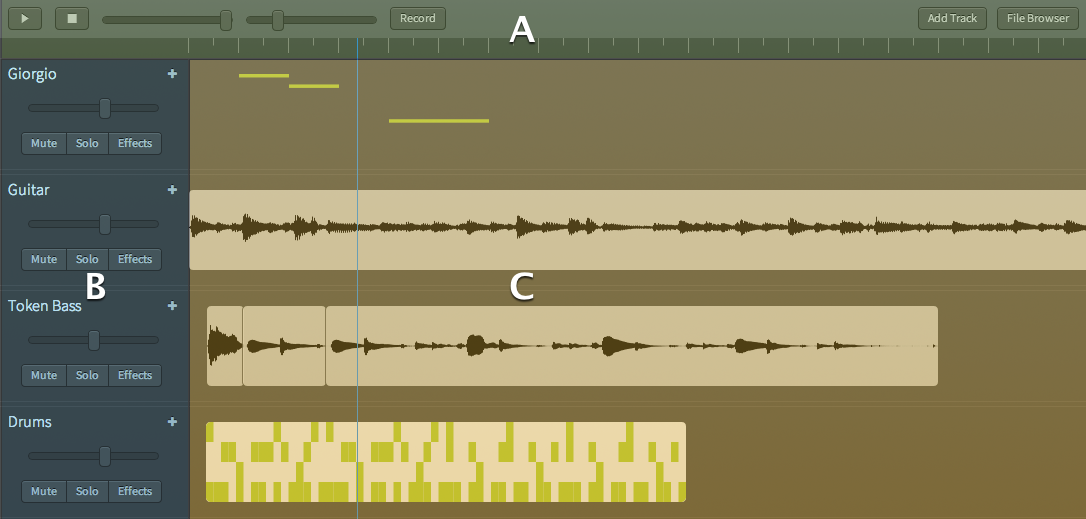
\includegraphics[width=\linewidth]{images/editor_overview_sections.png}}
    \caption[Editor Overview]{Editor Overview}
    \label{fig:editor-overview}
  \end{figure}

\end{landscape}
\newpage

\section{Structure}
\label{concept-overview}

The editor's structure is derived from Garageband, a DAW that is developed by Apple and which is part of their iLife software package\footnote{\url{http://www.apple.com/mac/garageband/}, last checked on 25/03/2014}. Garageband has a clear and easy to use user interface which is designed for both novice an expert users. The initial interface (\reffigure{fig:garageband-screenshot}) is simple and does not provide too many options. It can however be individualized by the user so that it fits the user's need and mental model. These options do not exist in the prototype of this thesis's editor, it just uses the same layout that is used in Garageband as well. The color palette for the editor's design is mainly inspired from Logic Pro X\footnote{\url{https://www.apple.com/logic-pro/}, last checked on 25/03/2014} (see \reffigure{fig:logic-screenshot}) and was built with the help of Adobe's Topcoat CSS package (\url{http://topcoat.io/}, last checked on 24/03/2014). Although the main structure was taken from Garageband, most other DAWs have a similar structure and it is easy for users to understand other DAWs, once they have become familiar with the concept of one of them (see \refchapter{ch:daw-apps}). 

The editor's user interface is split into three different parts (see \reffigure{fig:editor-overview}). Part A is the global control interface. The buttons on the left control the global playback of the arrangement. When the playback has been started, the blue line animates in the speed of the playback and acts as a progress indicator. It can also be controlled by clicking the vertical lines at the bottom of part A. A click on these lines causes the playback to jump to the selected position. The lines have different sizes to indicate time ranges. A longer line marks a second and a shorter line half a second. Next to the playback buttons are two range elements. The first one controls the master volume and the second one controls the zoom level. The zoom level influences the preview size of each of the arrangement's pieces. The button to the right of the range elements triggers the recording of the piece. Recording is only supported in real-time, so it works in the same way as tape recorders. When it is pressed, the playback starts, the button flashes red and the master output is recorded. The recording has to be stopped manually as well. After stopping the recording, the recorded file will be downloaded automatically. The button that says `Add Track' opens up a dialog that lets the user choose a type of track to add to the arrangement. The button that says `File Browser' opens up the file browser interface (see \refchapter{concept-import}).

Part B of the editor's layout contains the control panels for each of the tracks that were created by the user. Each track has an editable title, a volume control that only influences the current track's volume and it has buttons to turn on the mute or the solo mode of a track (see \refchapter{impl-tracks}). A third button `Effects' is also part of the control interface and it was designed to trigger an effects control panel for a track. Due to time limitations, this panel has not been implemented in the end. The `+' button in the upper right hand corner of the control panel adds a new piece to the track.

Part C shows previews for the individual pieces of the arrangement. The term pieces refers to audio pieces that have been created by using the editor's audio modules. Each track has a certain type and therefore only pieces of that type can be arranged in it. The different types of pieces and audio modules are explained in more detail in \refchapter{concept-modules}. The visual position of the previews determines their position in the arrangement and it can be changed by simply dragging them to the desired location. The properties of each piece can be changed by opening up their edit-interfaces that show up when they are double-clicked.

\section{Audio Modules}
\label{concept-modules}

Based on the capabilities of the Web Audio API (see \refchapter{ch:audio-theory}) and by looking at other DAW software, four different audio modules have been identified that build the foundation of a DAW. This chapter will show the prototypical web-based user interface for all four modules and it will explain their functionality.

\subsection{Recording}
\label{concept-recording}

\subsubsection{Preview}
\label{subsub:recording-preview}

The most basic element that needs to be in a DAW application is the recording functionality. It is essential that users can record and save audio signals e.g. from a microphone or a plugged in instrument like a guitar. The visual representation of a recording in all DAWs is the signal's waveform and therefore is also represented as a waveform in this editor as it can be seen in the `Guitar' and in the `Token Bass' track in \reffigure{fig:editor-overview}. It shows the amplitude alterations over time and indicates which part of a recording is louder than others. From that, the user can conclude which part of the recording is shown.

\subsubsection{Recording the signal}
\label{subsub:recording-ui}

\begin{figure}[htb]
  \centerline{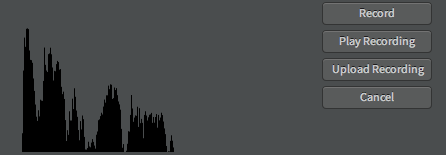
\includegraphics[width=\linewidth]{images/recording-a-signal.png}}
  \caption[Recording the signal]{Recording the signal}
  \label{fig:editor-recording-a-signal}
\end{figure}

\reffigure{fig:editor-recording-a-signal} shows the user interface for recording the user's input signal. The input could come from an external sound card, as well as from an internal microphone. The view is shown when the `+' button on a recording track is pressed. As soon as the user has agreed to give the application read access to the input signal, a visualization of the input signal is displayed that shows the frequency spectrum of the real-time data (see \refchapter{impl-recording-piece}). The user can initiate the recording by clicking the `Record' button which will flash red while recording. After finishing the recording, the `Play Recording' button plays the currently recorded bit and the `Upload Recording' button will upload the recorded file to the server and insert it into the current track.

\subsubsection{Editing a recording}
\label{subsub:recording-edit}

\begin{figure}[htb]
  \centerline{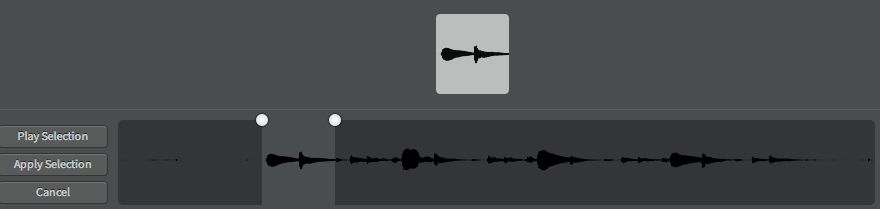
\includegraphics[width=\linewidth]{images/editing-a-recording.png}}
  \caption[Editing a recorded signal]{Editing a recorded signal}
  \label{fig:editor-editing-a-signal}
\end{figure}

In \reffigure{fig:editor-editing-a-signal} the edit interface for a recording is shown. Users have the ability to select a part from the recording which will then be used in the playback of the arrangement. In the example, only a small part from a longer recording is taken. This feature is especially useful to get rid of gaps from the start or the ending of a recording. A part is selected by dragging the two handles to the desired position of the recording. In order to check if the correct part has been selected, the user is able to playback the selection with the `Play Selection' button.

\subsection{Drum Machine}
\label{concept-drum}

\subsubsection{Preview}
\label{concept-drum-preview}

The drum machine preview can be seen in the track `Drum' in \reffigure{fig:editor-overview}. Each green rectangle stands for a beat in a pattern. The white parts are beats in a pattern that are not played. This kind of visualization is common in all DAW application (see \reffigure{fig:logic-screenshot} and \reffigure{fig:ableton-screenshot}). The width of the rectangles is defined by the amount of beats in a pattern and the zoom level of the editor. The height depends on the amount of different instruments in the specific drum kit.

\subsubsection{Editing}

\begin{figure}[htb]
  \centerline{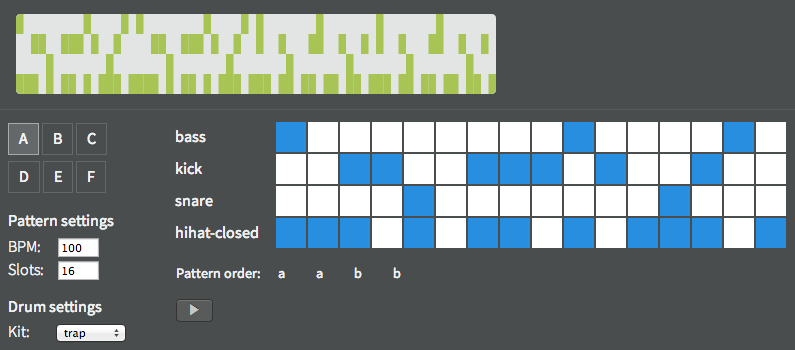
\includegraphics[width=\linewidth]{images/drum-edit.png}}
  \caption[Editing a drum loop]{Editing a drum loop}
  \label{fig:editor-editing-a-loop}
\end{figure}

\reffigure{fig:editor-editing-a-loop} shows the editing view for a drum machine piece. The grid to the right is used to activate and deactivate beats for the specific instruments. A blue rectangle means that the instrument will be played when this beat is being played and a white rectangle indicates a pause. The captions on the left of the grid represent the individual instruments. Again, this kind of user interface is very common among other DAWs as well and this one in particular is derived from FL Studio's\footnote{\url{http://www.image-line.com/flstudio/}. last checked on 25/04/2014} step sequencer (see \reffigure{fig:flstudio-screenshot}). The list of letters to the left stands for the amount of different patterns that can be created for a single drum machine piece. The order of patterns can be changed in the `Pattern Order' list by dragging patterns onto it and by using the order-arrows (only visible when hovered). This feature allows users to create complex pattern schemes in only one piece. A not so common feature that is supported in this editor is that for each pattern, a different speed (`BPM') and slot setting can be saved. This comes in handy when a complex pattern order needs a fill-in or a pause. The `Kit' select element gives the user the opportunity to change the drum kit, and therefore the sound for each beat. To the right there is also a play button which can be used to preview the drum pattern while editing it. The currently playing beat will be highlighted during the playback.

\subsection{Synthesizer}
\label{concept-synth}

\subsubsection{Preview}
\label{concept-synth-preview}

The preview of the synthesizer shows the individual tones and their length in a small version so that users can roughly see which tone will be played at which time. The vertical position of each tone is defined by its pitch (lower pitch - higher position) and its width is defined by the tone's length without an eventual release. It can be seen in the `Giorgio' track of \reffigure{fig:editor-overview}.

\subsubsection{Synthesizer Settings}
\label{concept-synth-settings}

\begin{figure}[htb]
  \centerline{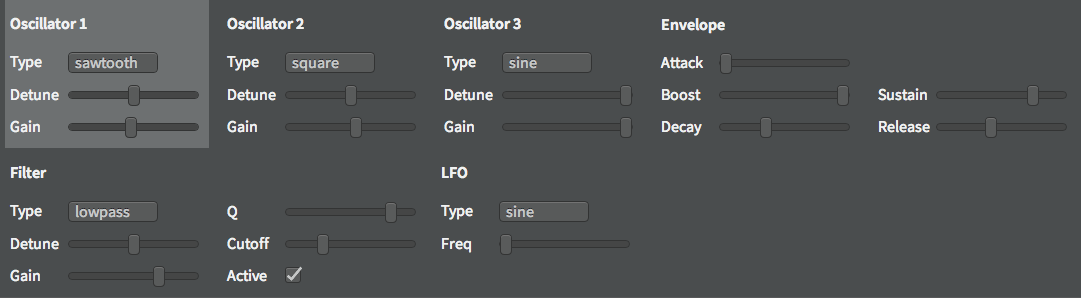
\includegraphics[width=\linewidth]{images/synth-settings.png}}
  \caption[The synthesizer's settings]{The synthesizer's settings}
  \label{fig:editor-concept-synth-settings}
\end{figure}

The synthesizer settings reveal that the synthesizer is a polyphonic synthesizer that features three individual oscillators for the sound generation. For each oscillator (`Oscillator 1-3'), the type of wave, the detune settings and the gain can be set. Detune is used to detune the pitch of the oscillator so that a more rich sound can be created. The detune settings allow an oscillator to be pitched an octave up and down. In the envelope settings, all classic parameters of an ADSR envelope can be defined (see \refchapter{sec:adsr-envelope}). The boost parameter is used to define the peak volume before the decay kicks in. The `Filter' form lets users choose and fine-tune a filter that will be used to shape the sound of the three oscillators. It can be toggled by ticking the `Active' checkbox. In the `LFO' section, an LFO (see \refchapter{sec:webaudio-synth}) can be activated and set to the desired sound. All sections will be highlighted when they are hovered so that the user always knows which parameters belong to which module of the synthesizer.

\subsubsection{Notes Grid}
\label{concept-synth-grid}

\begin{figure}[htb]
  \centerline{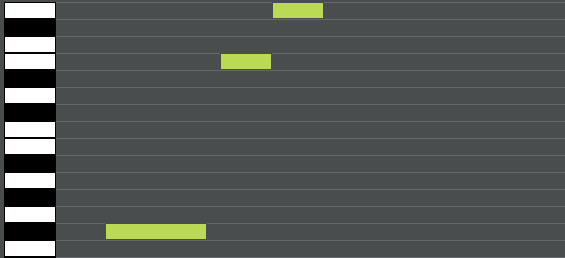
\includegraphics[width=\linewidth]{images/notes-grid.png}}
  \caption[The notes grid]{The notes grid}
  \label{fig:editor-concept-notes-grid}
\end{figure}

The notes for a synthesizer piece can be edited from the user interface that is shown in \reffigure{fig:editor-concept-notes-grid}. Similarly to the beats grid of the drum machine piece, the notes grid shows the notes on the right side. Each note can be dragged around to change its position in time and it can be deleted by double clicking it. A note is added to the grid by double clicking a note line. Its length can be changed by dragging its right edge. On the left, all notes of the keyboard are shown. Users are able to preview a note by playing it on the computer keyboard. The corresponding note will be played back and then highlighted in the user interface. The playback of all notes can be triggered using a play button at the bottom.

\subsection{Import \& File Browser}
\label{concept-import}

\begin{figure}[htb]
  \centerline{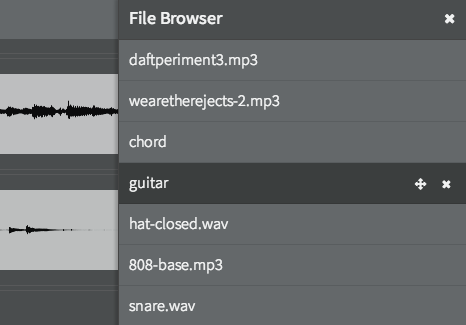
\includegraphics[width=.68\linewidth]{images/file-browser.png}}
  \caption[The file browser]{The file browser}
  \label{fig:editor-concept-file-browser}
\end{figure}

The fourth essential audio module that is present in every DAW is the ability to upload arbitrary sound files and use them in an arrangement. The editor supports this as well and audio files can be uploaded by dragging them onto recording tracks. They will be uploaded to the server automatically and then added to the file browser which can be seen in \reffigure{fig:editor-concept-file-browser}. All recordings and uploaded files will be listed there. In the figure, the `guitar' file is selected. The name can be edited in place and the file can be added to tracks by dragging it at the drag handle. It can also be deleted by using the `delete' button to the right.

\section{Synchronization}
\label{concept-synchronization}

All operations on pieces will be synchronized between all participating clients in real-time. The algorithm that realizes the synchronization has been described in \refchapter{ch:sync-theory} and its implementation will be described in \refchapter{impl-sync-algorithm}. The visual impact of the synchronization is minimal. Since the synchronization should happen in real-time without user interaction, the remote changes can be applied to the pieces and their edit interfaces while the editor is in use. If for example, the position of a piece is changed because user A dragged the piece to another position, the piece will also jump to this position in user B's editor. Also, all previews and edit-interfaces will be updated accordingly in real-time (e.g. the beats grid), so that even when two users are editing the same piece, the other user's changes can be taken into account and users can truly work on all pieces collaboratively. However, changes will only be applied when operations are finished and no in-between states are synced between the clients. For example, when a user edits the title of a track. The change of the title will only be sent to the server once the user has finished editing the title. The same applies to position changes of pieces. The position of the piece while dragging it will not be synchronized until the user has released the dragged element. In-between states are not synced because they can distract the other users while they are editing other parts of the arrangement.